\begin{figure}[htbp]
\centering
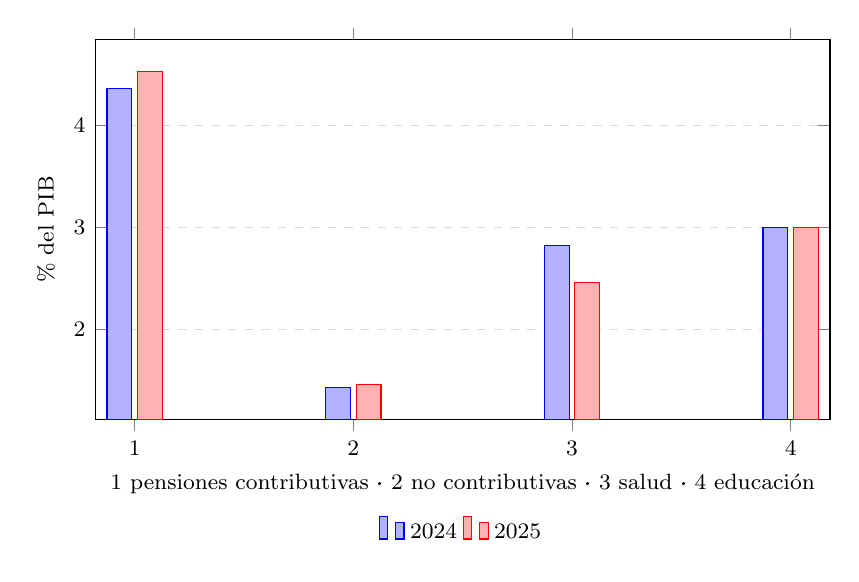
\begin{tikzpicture}
\begin{axis}[
  width=0.9\textwidth, height=6.4cm,
  xlabel={1 pensiones contributivas · 2 no contributivas · 3 salud · 4 educación}, ylabel={\% del PIB},
  legend style={font=\footnotesize, at={(0.5,-0.24)}, anchor=north,
                 legend columns=-1, draw=none},
  tick label style={font=\footnotesize},
  label style={font=\footnotesize},
  x tick label style={/pgf/number format/1000 sep={}},
  ymajorgrids=true, grid style={dashed, gray!30},
  enlarge x limits=0.06,
  cycle list={{solid,mark=*}, {dashed,mark=square*}, {dotted,mark=triangle*}, {dashdotted,mark=diamond*}},
  ybar, bar width=9pt,
  xtick=data,
]
\addplot+ coordinates {(1,4.36) (2,1.43) (3,2.82) (4,3.0)};
\addlegendentry{2024}
\addplot+ coordinates {(1,4.53) (2,1.46) (3,2.46) (4,3.0)};
\addlegendentry{2025}
\end{axis}
\end{tikzpicture}
\caption{La tríada de transferencias de ciclo de vida, 2024 y 2025}
\label{fig:F13_1}
\par\vspace{2pt}\footnotesize Fuente: elaboración propia del ITED con los analíticos del PEF aprobado 2024 y 2025. Mismos perímetros que los capítulos 5, 6 y 7.
\end{figure}
